\documentclass{article}
\usepackage{graphicx}

\title{Are You Rational?}
\author{Edward Yu}

\begin{document}

\maketitle
There is an old joke about Homo Economicus, a purely rational decision-making human that always seeks to maximize profit (to use fancy words, ``utility’’).
Of course, Homo Economicus is not Homo Sapiens, nor are we Mr. Spock; we are not purely logical beings all the time.
\begin{center}
    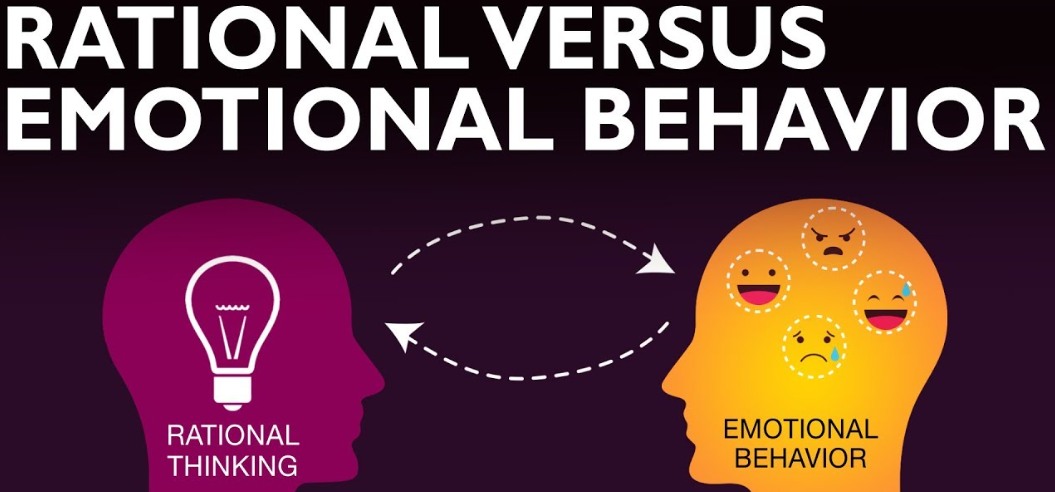
\includegraphics[scale=0.4]{images/rational.png}
\end{center}

We think we strive for logical decision-making during our most important decisions, yet we still are quite fallible. Here are some of my favorite examples of when human ``rational’’ decision-making goes awry.

\textbf{The Allais Paradox:} An eccentric billionaire offers you a choice between two gambles:
\begin{enumerate}
\item \$1 million, guaranteed, or
\item A 1\% chance of nothing, 89\% chance of getting \$1 million, and \$5 million otherwise?
\end{enumerate}
Most people choose the former over the latter: that 1\% chance of zero reward in the second scenario is intimidating, and perhaps not worth the (improbable) possibility of a \$5 million bonus.

Now, consider another choice. Would you rather take:
\begin{enumerate}
\item \$1 million with 11\% probability and nothing otherwise, or
\item \$5 million with 10\% probability and nothing otherwise?
\end{enumerate}
Once again, the decision is clear: there’s basically no distinction between 10\% and 11\%, and of course \$5 million is much more preferable to \$1 million, so we’ll go with the second choice.

The careful reader will already observe the problem: the two scenarios presented above are secretly the same scenario!
To get from the second scenario to the first one, the billionaire gives us an extra \$1 million with 89\% probability in both options. This paradoxically causes us to change our mind! It's as if we prefer apples to bananas, yet prefer an banana (plus a dollar bill) to an apple (plus a dollar bill).

So, why does the extra 1\% make such a difference? There are many formulations of the mathematically-reasoning human subconscious that seek to explain this away---``risk aversion'' and ``loss aversion'' are common related terms that you'll hear a lot on this context---but most of us are still faced with the gut-punch conclusion that we ``rationally'' made an inconsistent choice.

\textbf{The St. Petersburg Paradox:}
The eccentric billionaire is back! This time, they're going to play the following game with you. They throw in \$1 into the pot, and you repeatedly flip a coin. Every time the coin lands heads, the value of the pot doubles, and when the coin lands tails for the first time, you win everything in the pot.

\begin{center}
    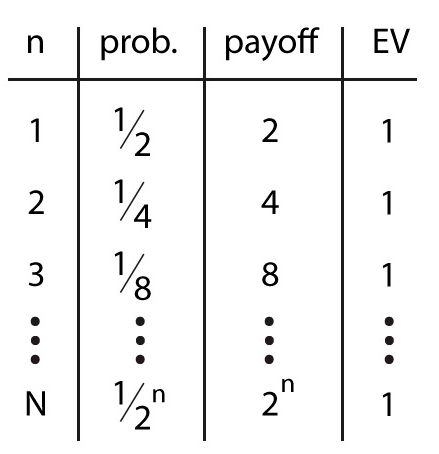
\includegraphics[scale=0.6]{images/st_petersberg.png}
\end{center}

So, for example, if you tossed three heads in a row followed by tails, you'd win \$8.
How much would you be willing to pay to play this game?

Supposedly, you should be willing to pay any amount of money: the expected payoff (your average winnings) is infinite! You can check this with a simple expected-value calculation:
\[1\times\frac12 + 2\times\frac14 + 4\times\frac18 + \cdots \]
\[= \frac12 + \frac12 + \frac12 + \cdots = \infty.\]

But before you sell all of your possessions to purchase a ticket (don't try this at home), keep in mind that the amount you'll win is probably vanishingly small: there's a 75\% chance you'll walk away with \$2 or less! So most of the value of the game comes from magnificently large payoffs with vanishingly small probabilities---in this case it's common sense that has to save us from the perils of expected-value-maximizing calculations.

\textbf{Newcomb’s Paradox:} The billionaire has one final challenge for you. They show you two boxes, labeled A and B, and you can choose to take either box B only, or both boxes A and B.
They also have an infallible crystal ball, which will predict your action.

You see the following in each box:
\begin{itemize}
    \item Box A is transparent and always contains a visible \$1,000.
    \item Box B is opaque (you can't see inside), but its content has been set by the predictor:
    \begin{itemize}
    \item If the predictor has predicted that the player will take both boxes A and B, then box B contains nothing.
    \item If the predictor has predicted that the player will take only box B, then box B contains \$1,000,000.
    \end{itemize}
\end{itemize}
Should you take B only (known as ``one-boxing''), or both A and B (known as ``two-boxing'')?

It has been remarked that to almost everyone, it is perfectly obvious what should be done, but ``the difficulty is that these people seem to divide almost evenly on the problem, with large numbers thinking that the opposing half is just being silly.''
I'll leave the analysis of this last one to you, since philosophers even today are divided on which option to take. Enjoy---and remember, always, that you might not always be thinking rationally!
\end{document}